\documentclass[a4paper,12pt]{amsart}

\usepackage[spanish]{babel}
\usepackage[style=ieee]{biblatex}
\addbibresource{./references.bib}
\usepackage[utf8]{inputenc}
\usepackage[margin=2cm]{geometry}
\usepackage[labelfont=bf,textfont=it]{caption,subcaption}
\usepackage{amsmath,amssymb,amsfonts}
\usepackage{graphicx,fancyhdr}
\usepackage{csquotes}

\author{José Luis Aguilar Charfén}
\date{\today}
\title{Objetivos de Desarrollo Sostenible: proyecto de Machine Learning}




\begin{document}
    \begin{abstract} % ! TODO
        Este reporte muestra la predicción del SDG Index Score en términos de 
        los primeros dos Objetivos de Desarrollo Sostenible (SDGs). Se discute 
        y argumenta la metodología seguida, y se evalúa el modelo con X métricas que luego se discutirán ajajajajaj
    \end{abstract}
    \maketitle

    \section{Introducción}

    Los Objetivos de Desarrollo Sustentable son 17 metas que se acordaron en la 
    Organización de las Naciones Unidas (ONU) en 2015 \cite{united_nations_development_programme_sustainable_nodate-1}
    como una llamada a la acción para proteger al planeta y asegurar que para
    2030 la población disfrute de paz y seguridad. 

    Estos objetivos varían desde reducir la pobreza, hasta temas de salud, 
    equidad de género, higiene, crecimiento económico, energía y cuidado al medio ambiente. 
    Cuando se consideran todos los diferentes objetivos, entonces se construye el 
    SDG Index Score, que califica el progreso de un país en las 17 metas. Para 
    este reporte, se enfocará en las primeras dos: \emph{fin de la pobreza}, y \emph{hambre cero}.

    		
    \section{Metodología}

    Los datos utilizados son de las siguientes categorías, descritas brevemente:
    \begin{enumerate}
        \item \emph{Poverty headcount ratio at \$1.90/ day (\%)}: Cuenta el porcentaje de gente que vive con menos de 1.90 dólares al día. Mientras mayor sea, indica un mayor nivel de pobreza.
        \item \emph{Poverty headcount ratio at \$3.20/day (\%)}: Cuenta el porcentaje de gente que vive con menos de 1.90 dólares al día. Se espera que esté fuertemente correlacionada con la variable anterior.
        \item \emph{Poverty rate after taxes and transfers (\%)}: Cuenta la cantidad de gente que su ingreso cae por debajo de la línea de probreza, tomada como el 50\% del actual ingreso disponible después de impuestos y transferencias contadas como pagos a escuela o arreglos de alojamiento. Esta métrica solo está disponible para países de la OCDE. \cite{noauthor_income_nodate} 
        \item \emph{Prevalence of undernourishment (\%)}: Es el porcentaje de la población que su consumo alimenticio es insuficiente para proveer los niveles energéticos necesarios para mantener una vida activa y saludable.
        \item \emph{Prevalence of stunting in children under 5 years of age (\%)}: Se refiere al porcentaje de la población infante que sufre de retraso en el crecimiento.
        \item \emph{Prevalence of wasting in children under 5 years of age (\%)}: Se refiere al porcentaje de la población que es demasiado delgado para su altura y resulta por incapacidad de ganar peso o por bajar muy rápido.
        \item \emph{Prevalence of obesity, BMI $\ge$ 30 (\% of adult population)}: Se refiere al porcentaje de gente que está por encima de un índice de masa corporal por arriba de 30\footnote{Pueden existir críticas por si es una métrica válida o útil, pero queda por fuera del alcance de este proyecto.}.
        \item \emph{Human Trophic Level (best 2-3 worst)}: Nivel trófico del humano. Se refiere a la posición que ocuparía en una pirámide alimenticia. Un valor de 1 sería un productor primario, como una planta, y un nivel de 5 sería un depredador ápice, por ejemplo un oso polar o un esquimal. Se puede calcular con la siguiente ecuación\cite{bonhommeau_eating_2013}: 
        \begin{equation}
            N_{T_i} = 1 + \sum_j\left(N_{T_j}y_{ij}\right) 
        \end{equation}
        Donde $N_{T_i}$ es el nivel trófico de la población $i$, $N_{T_j}$ el de la presa $j$, y $y_{ij}$ es la fracción de la presa $j$ en la especie $i$. Sin embargo, la mayoría de los países se encuentran con un nivel entre 2 y 3. No puede ser menor a 2 porque no somos productores primarios. Usualmente se interpreta como mejor que sea menor el nivel trófico porque significa que la energía y recursos usados para producir la comida – por efectos de la eficiencia de transferencia de biomasa, que es aproximadamente del 10\% \cite{noauthor_calculating_nodate} – son menores.
        \item \emph{Cereal yield (tonnes per hectare of harvested land)}: Es el rendimiento de producción de cereales. Usualmente, una mayor cantidad significa que la tierra es más fértil. 
        \item \emph{Sustainable Nitrogen Management Index (best 0-1.41 worst)}: Esta métrica combina dos medidas de eficiencia en la producción agrícola: la eficiencia de uso de nitrógeno, y eficiencia de uso de tierras. La eficiencia de uso de nitrógeno se define como la fracción de entradas de nitrógeno que termina en los productos, y normalmente debe estar entre 0 y 1, con valores normalmente entre 0.5 y 0.9\cite{zhang_sustainable_2019}, indicando uso eficiente uso del nitrógeno, pero puede ser mayor a 1 si sale de la tierra, eliminando recursos. Combina además qué tanto se produce por hectárea, y la métrica construida por Zhang y Davidson idealmente alcanza 0, mostrando este número un alto rendimiento del uso de nitrógeno y de uso de tierras. 
        \item \emph{Yield gap closure (\% of potential yield)}: Indica en porcentaje el rendimiento potencial en los tres principales cultivos, ponderados por la importancia de cada cultivo en términos del área que ocupa. Solo está disponible para países de la OCDE. Mientras mayor sea su valor indica un uso más eficiente de tierra. 
        \item \emph{Exports of hazardous pesticides (tonnes per million population)}: Toma el valor promedio de los últimos 5 años de las exportaciones de pesticidas vistos como materiales peligrosos; por ejemplo, el glifosato (o en general los pesticidas organofosfatados).
    \end{enumerate}

    Debido a que tanto la tasa de pobreza medida con el ingreso disponible, como 
    la cerradura de la brecha del rendimiento de plantas reportadas en el 
    conjunto de datos utilizado solamente están disponibles para la OCDE, 
    existen tres principales posibilidades para tratarlos. La primera consiste 
    en modelar diferente para la OCDE e incluir estos valores, y otro modelo sin 
    considerar estas variables para el resto del mundo\footnote{Alternativamente, 
    puede hacerse un modelo por continente, pero se deja como propuesta meramente}.
    Como segunda opción, pueden imputarse sus valores con alguna técnica, suponiendo 
    que sus valores serán parecidos a los de la OCDE. Puede, por ejemplo, imputarse
    con la media, o la mediana. Como tercera opción, pueden removerse como 
    variables, reconociendo que posiblemente, debido a que la situación sociopolítica 
    y económica de los países de la OCDE es distinta a la del resto del mundo, 
    entonces la información que se pueda extraer de los valores imputados de esta 
    variable introduzcan un sesgo que no puede observarse fácilmente, y afectar
    las predicciones de maneras no deseables (por ejemplo, falsamente sugiriendo
    una relación más fuerte de la que existe realmente, o al revés, que no sea 
    significativa).

    Adicionalmente, se decide eliminar como valor para predecir a Eswatini, debido a que 
    en el nivel trófico muestra un valor atípicamente alto (4), mucho mayor al 
    siguiente país que es Islandia, con un valor de 2.583. Además, un nivel 
    trófico de 4 supone que el consumo de alimentos es básicamente de animales 
    carnívoros, o por su contra, que casi no existen plantas en la dieta de la 
    población, que no coincide con la dieta usual de la mayoría de los países. 
    Además de ser atípicamente alto, de incluirse en el modelo, puede provocar 
    un apalancamiento muy grande, afectando fuertemente al valor del estimador. 

    Debido a que no todos los países tienen un SDG Index Score, no se consideran
    para entrenamiento ni validación ni prueba a estos países. Sin embargo, sí 
    se predicen sus valores dadas las variables usadas para construir los primeros 
    dos SDGs.

    Para construir el modelo, se realiza un análisis de correlación de variables, 
    y se observan tanto las distribuciones como las correlaciones con gráficos 
    por pares de variables. Posteriormente, se transforman las variables con la 
    transformación Yeo-Johnson \cite{yeo_new_2000}, preferida sobre la de Box y Cox por la presencia 
    de valores 0 en las variables. Posteriormente, se imputan los valores con 
    metodología de vecinos más cercanos \cite{beretta_nearest_2016}. Después, 
    se codifican las regiones usadas para el SDG Index por un método one-hot. 
    Una vez transformadas las variables de estas maneras, se comparan un modelo 
    de mínimos cuadrados ordinarios, regresión Ridge, y Lasso, ajustando sus 
    regularizaciones por validación cruzada, y se evalúa si se encuentra 
    sobreajustado comparando el error cuadrático medio del conjunto de datos 
    de entrenamiento con uno de prueba por separado, corriendo 20 veces el 
    experimento y promediando los valores.

    Las decisiones de construcción del modelo y justificaciones se discuten a
    mayor profundidad en la sección de resultados y conclusión.

    \section{Resultados y discusión}
    Se observan en la figura \ref{fig:correlations} y \ref{fig:corr_regions} las 
    correlaciones que existen entre las distintas variables de los datos. Puede observarse 
    que aquellas asociadas con la pobreza tienden a estar negativamente correlacionadas 
    con el índice SDG, lo cual hace sentido, y que están fuertemente correlacionadas entre 
    sí. Al descomponer las correlaciones para que se observen por región, puede 
    verse que existen ciertas diferencias en las correlaciones entre tipos de datos, siendo 
    más fuertes por ejemplo en Oceanía, que en Latinoamérica. 
    \begin{figure}[!ht]
        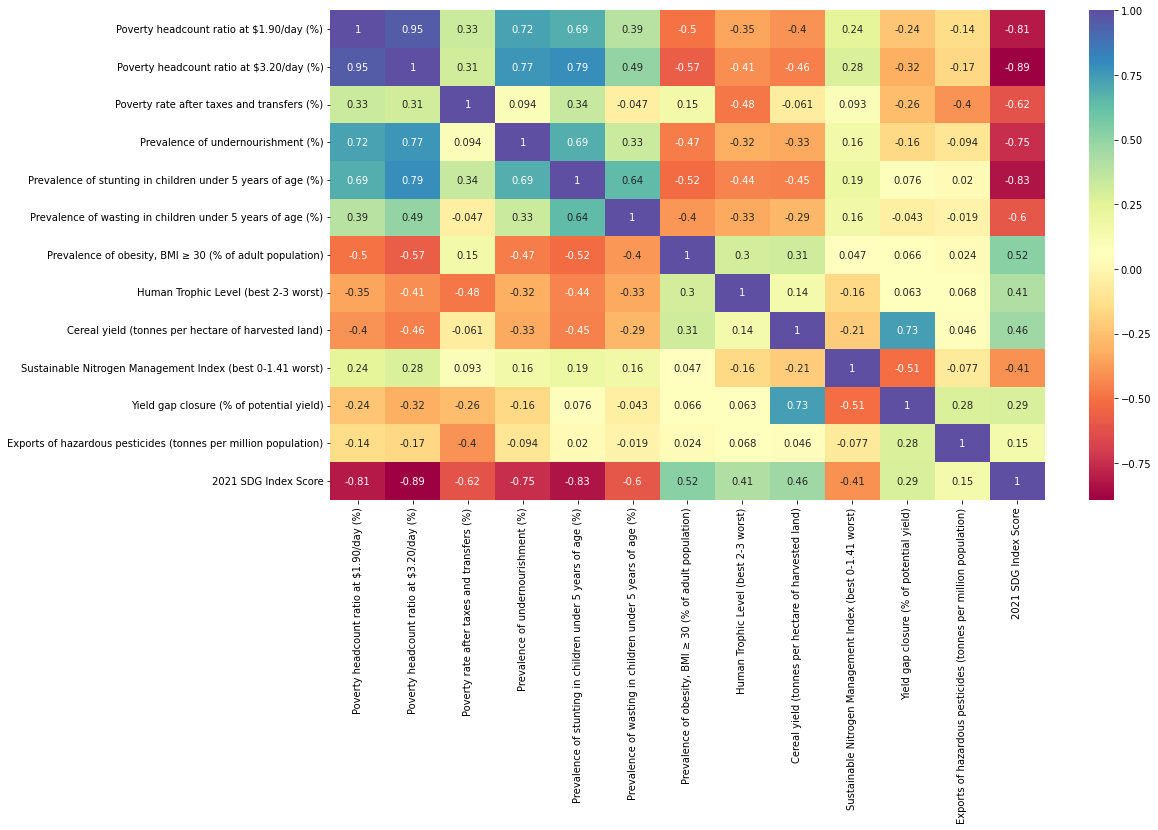
\includegraphics[width=\linewidth]{Images/Corr_todos.png}
        \caption{Matriz de correlación de las variables numéricas del modelo.}\label{fig:correlations}
    \end{figure}

    \begin{figure}[!h]
        \centering
        \begin{subfigure}{0.49\textwidth}
            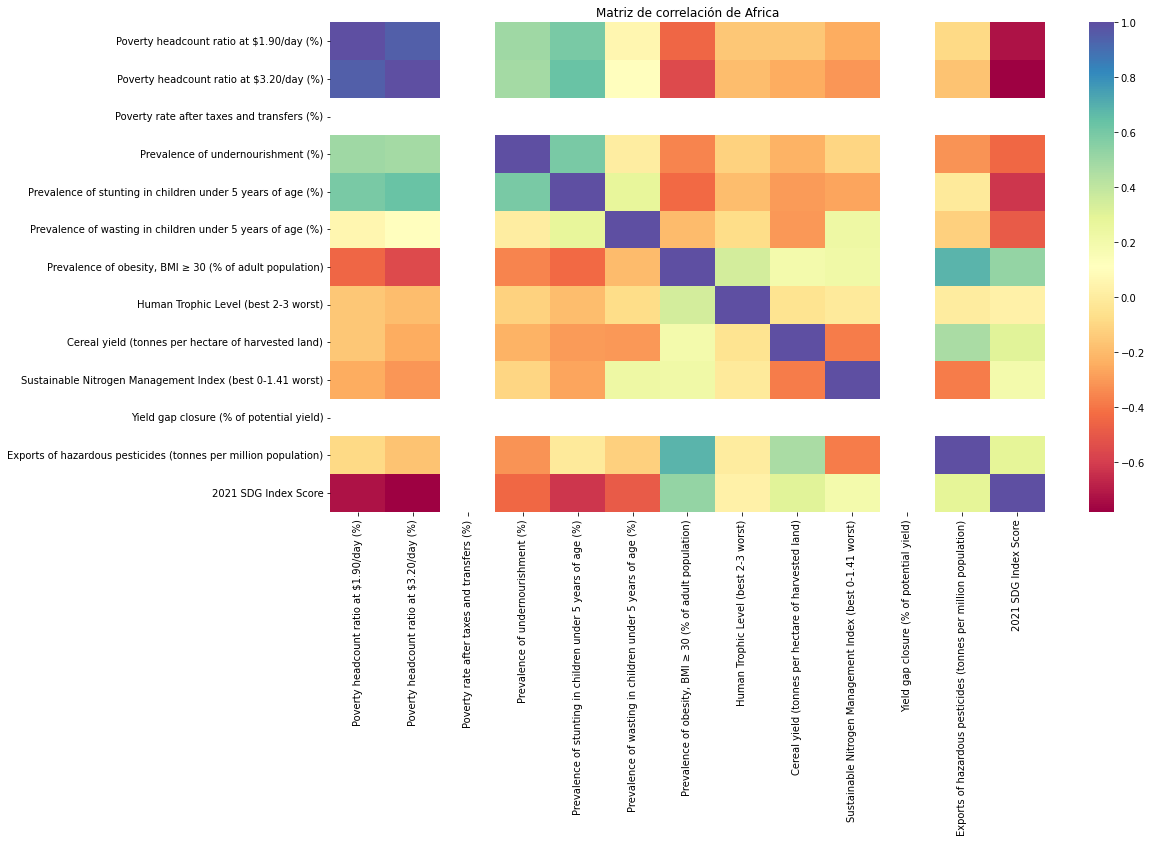
\includegraphics[width=\linewidth]{Images/Corr_africa.png}
        \end{subfigure}
        \begin{subfigure}{0.49\textwidth}
            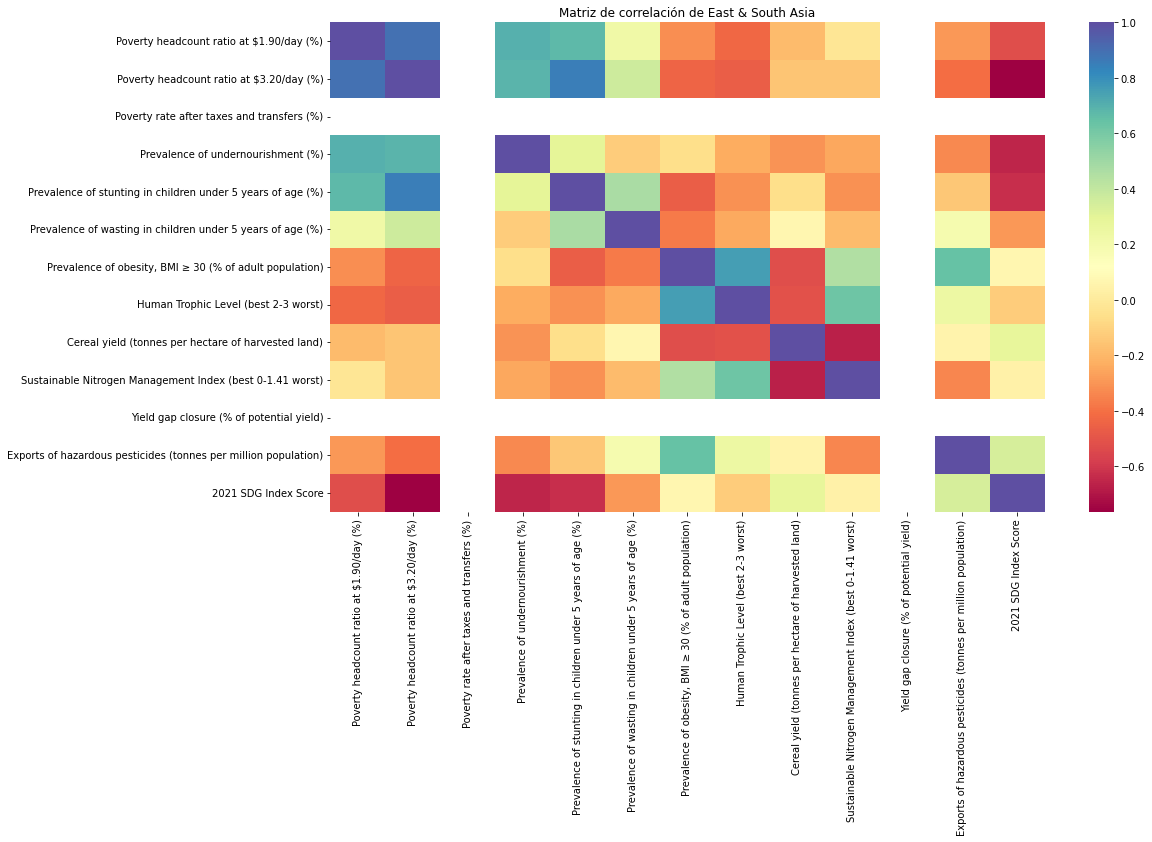
\includegraphics[width=\linewidth]{Images/Corr_asia.png}
        \end{subfigure}
        \begin{subfigure}{0.49\textwidth}
            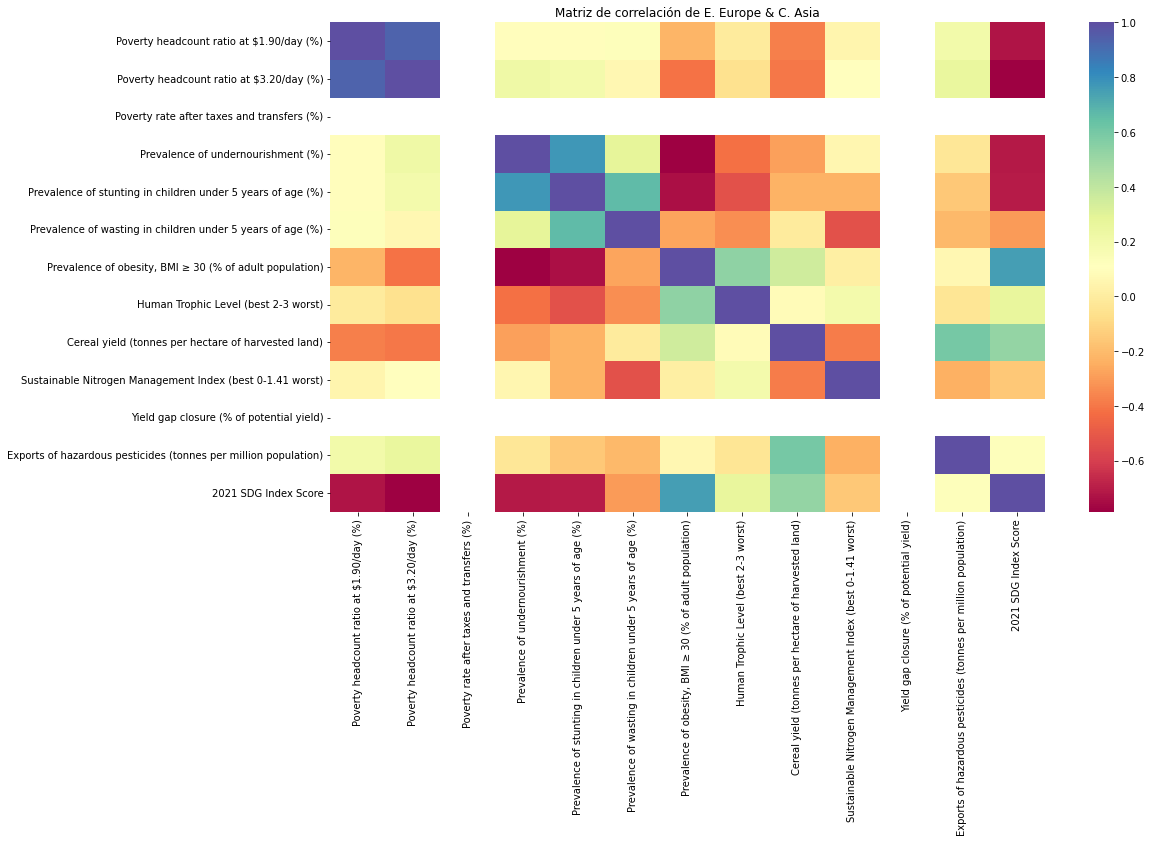
\includegraphics[width=\linewidth]{Images/Corr_europe.png}
        \end{subfigure}
        \begin{subfigure}{0.49\textwidth}
            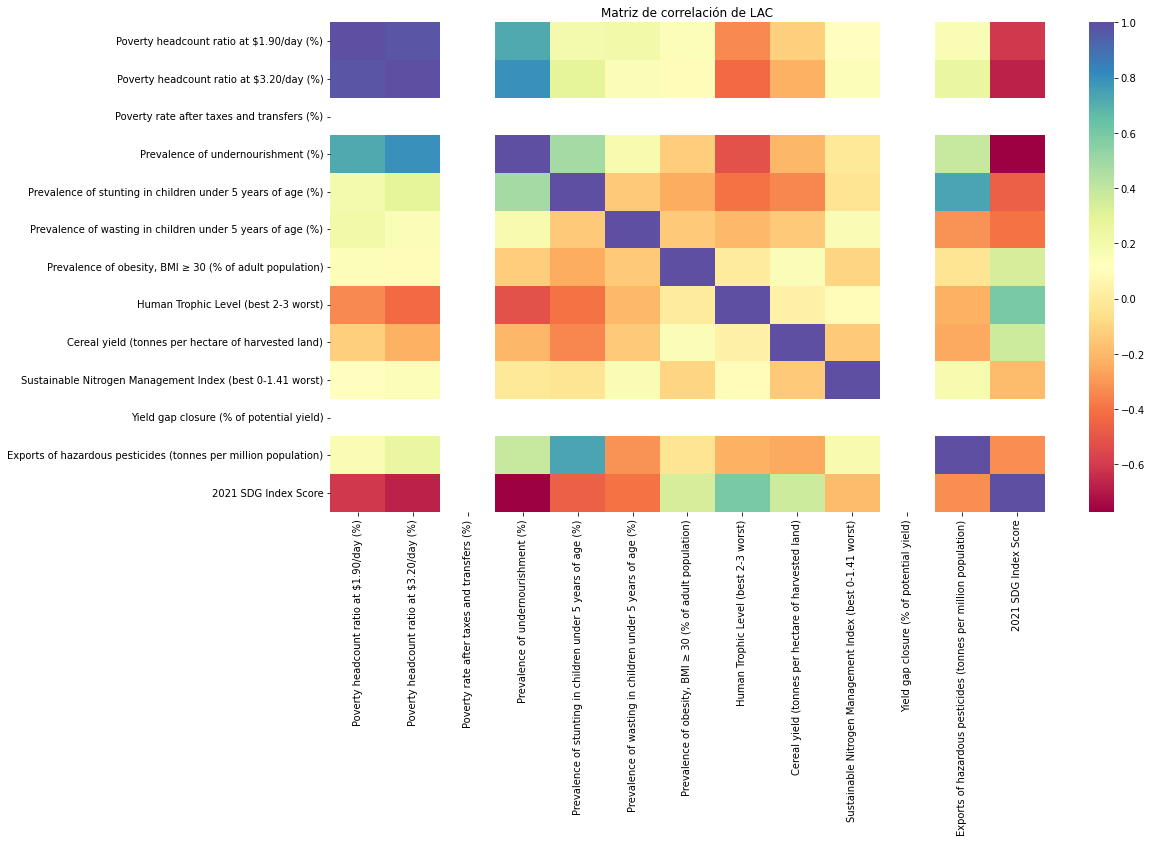
\includegraphics[width=\linewidth]{Images/Corr_LAC.png}
        \end{subfigure}
        
        \centering
        \begin{subfigure}{0.49\textwidth}
            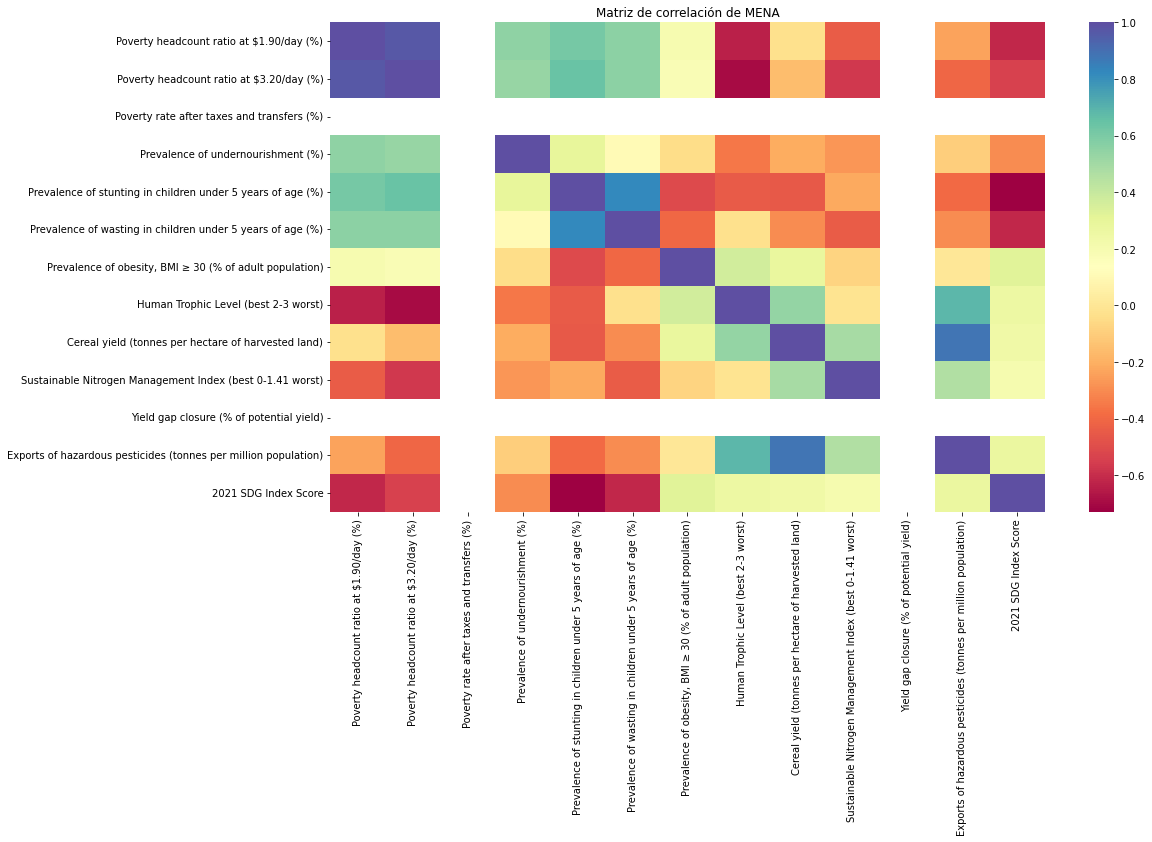
\includegraphics[width=\linewidth]{Images/Corr_MENA.png}
        \end{subfigure}
        \begin{subfigure}{0.49\textwidth}
            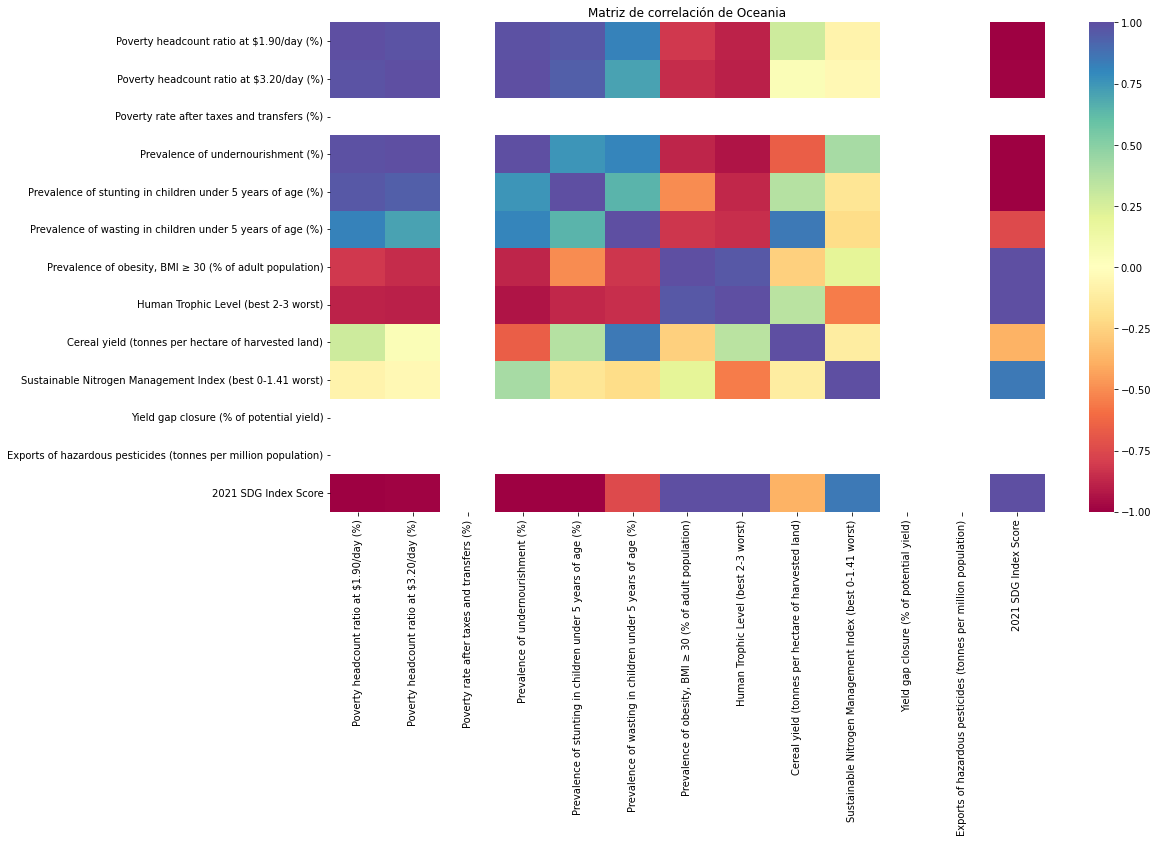
\includegraphics[width=\linewidth]{Images/Corr_oceania.png}
        \end{subfigure}
        \begin{subfigure}{0.49\textwidth}
            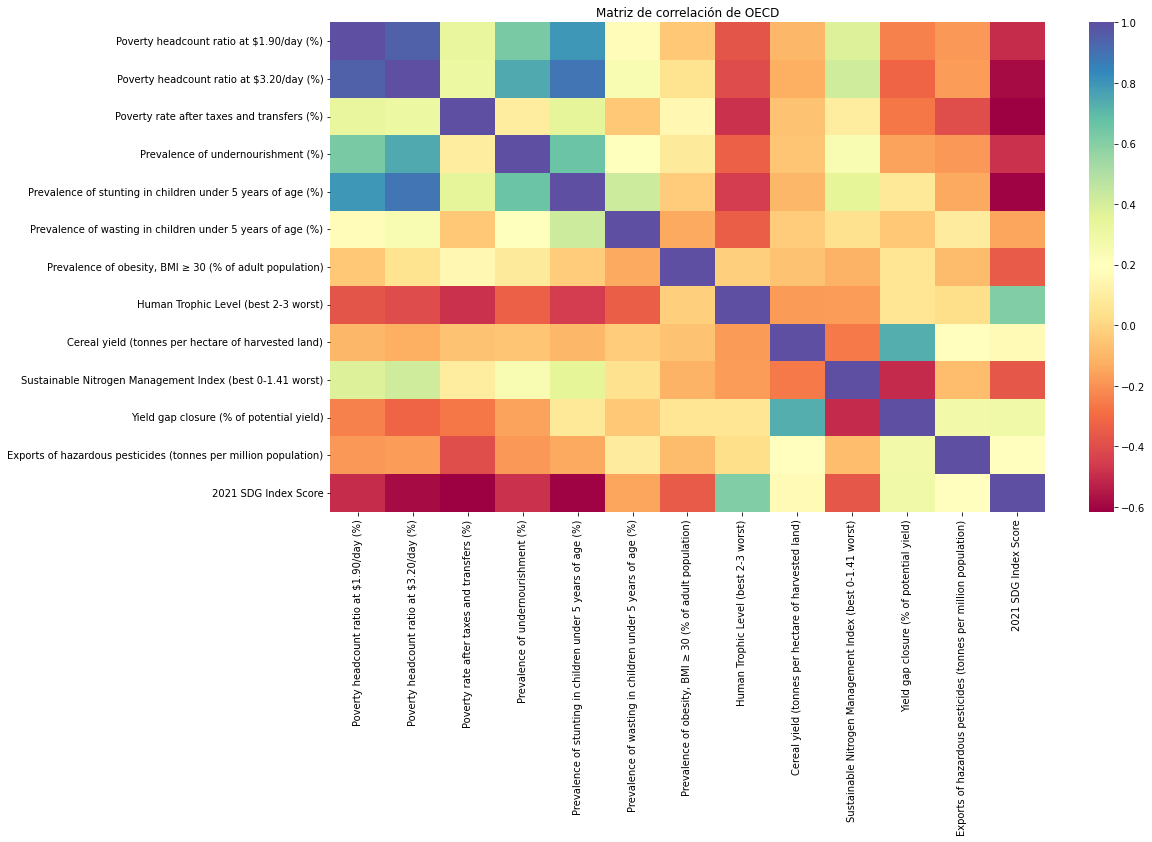
\includegraphics[width=\linewidth]{Images/Corr_oecd.png}
        \end{subfigure}
        \caption{Matrices de correlación de variables numéricas del modelo por región usada para calcular SDGs.}\label{fig:corr_regions}
    \end{figure}

    Es notable mencionar que no necesariamente se cumple el que las distribuciones estén idénticamente 
    distribuidas por región. Debido a esta dependencia, se decide incluir en el
    modelo la región de la que viene como variable predictora; para ejemplificar, 
    se ve claramente la diferencia en distribuciones en la figura \ref{fig:HTI},
    lo que sugiere que es una buena idea incluirse. Debe reconocerse, sin embargo, 
    que aunque exista una relación, no implica causalidad, y el modelo meramente 
    indica su presencia. Debe tenerse en cuenta que es un modelo reducido, y que 
    en uno completo en principio no debería usarse, bajo la interpretación de que 
    el pertenecer a una región favoreciera tu puntuación\footnote{Vale la pena recordar que la metodología usada para calcular el score es promediar los puntajes de cada uno de los SDGs\cite{united_nations_development_programme_sustainable_nodate}}.

    \begin{figure}[h!]
        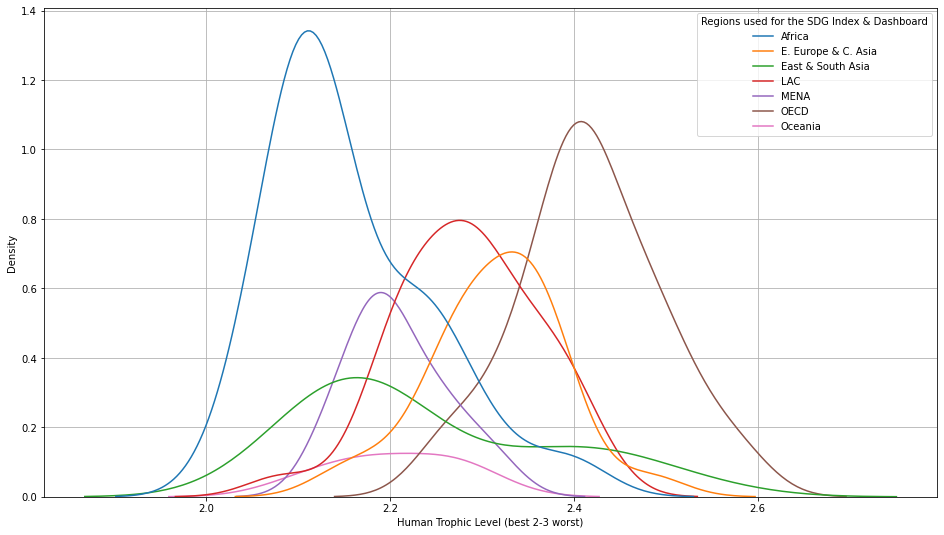
\includegraphics[width=\linewidth]{Images/Ejemplo_distribuciones.png}
        \caption{Distribuciones del índice trófico humano por región.}\label{fig:HTI}
    \end{figure}

    En la figura \ref{fig:distributions} se observan las distribuciones cumulativas 
    empíricas de los datos utilizados para el análisis. En los datos no transformados, 
    puede observarse que el común supuesto de normalidad no se respeta, por lo que 
    existe que los puntos que se encuentren en la cola de la distribución sean muy 
    influyentes en los valores de los parámetros usados para estimar, en particular 
    si son datos atípicos. Debido a esto, se propone una transformación de los datos
    con la técnica de Yeo-Johnson \cite{yeo_new_2000}, favorecida sobre la de 
    Box y Cox por la presencia de valores 0 en los datos. Puede notarse que con 
    esta transformación se ven mucho más cercanos a una distribución normal. 

    \begin{figure}[h!]
        \begin{subfigure}[t]{0.49\linewidth}
            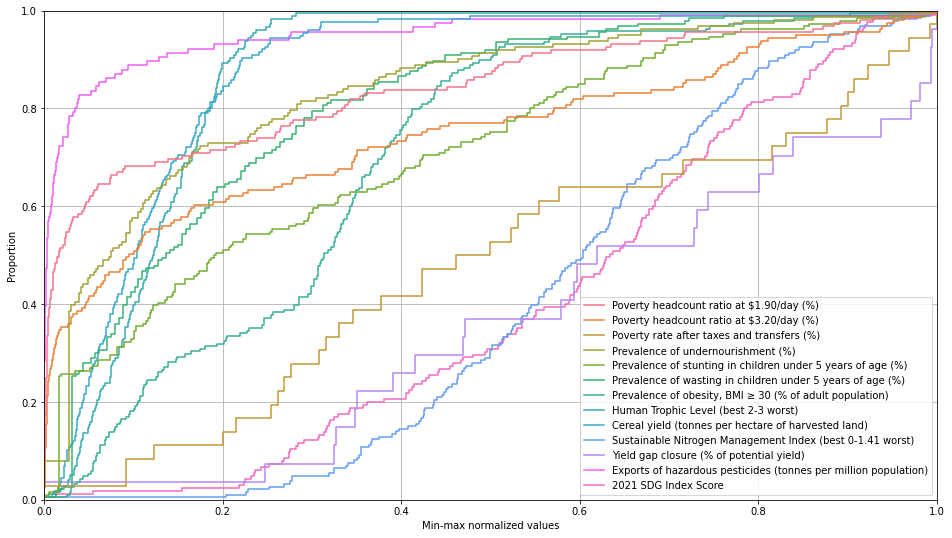
\includegraphics[width=\linewidth]{Images/CDF_no_transformado.png}
            \caption{Distribuciones de datos no transformados.}
        \end{subfigure}
        \begin{subfigure}[t]{0.49\linewidth}
            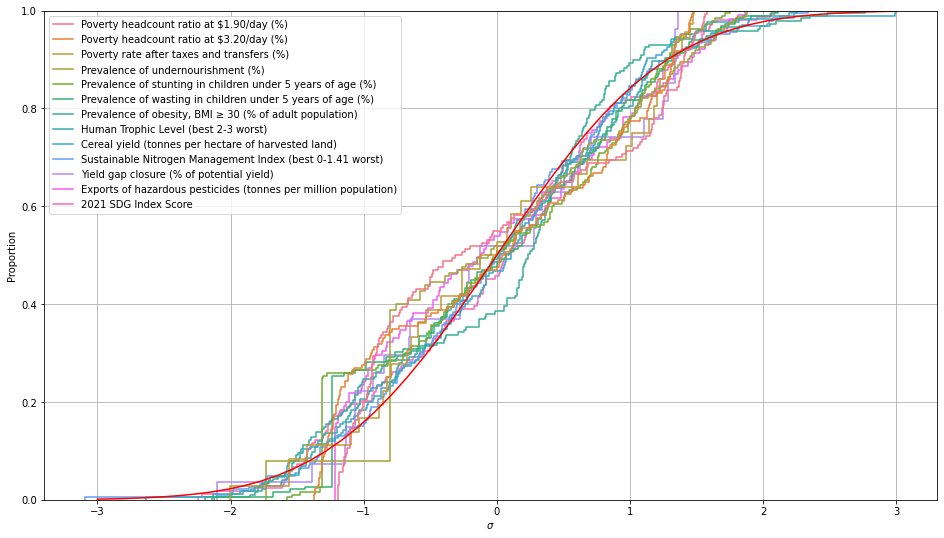
\includegraphics[width=\linewidth]{Images/CDF_transformado.png}
            \caption{Distribuciones de datos transformados. En rojo: distribución normal acumulada con media de 0 y varianza de 1}
        \end{subfigure}
        \caption{Distribuciones de datos antes y después de transformar.}\label{fig:distributions}
    \end{figure}

    En la figura \ref{fig:pis} se observan las porporciones de descomposición de 
    varianzas para las variables numéricas. Puede notarse que en los datos originales 
    existe colinealidad entre las dos primeras variables, que son las que indican 
    la cantidad de gente que vive debajo de cierto nivel de pobreza, pero son las únicas 
    que presentan una colinealidad relativamente fuerte. Existen otras más débiles, 
    pero resultan poco preocupantes.

    \begin{figure}[!ht]
        \begin{subfigure}{0.49\linewidth}
            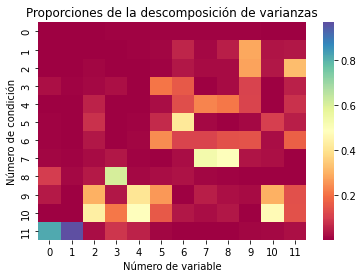
\includegraphics[width=\linewidth]{Images/VDM.png}
            \caption{Proporción de descomposición de varianzas solo para variables numéricas.}
        \end{subfigure}
        \begin{subfigure}{0.49\linewidth}
            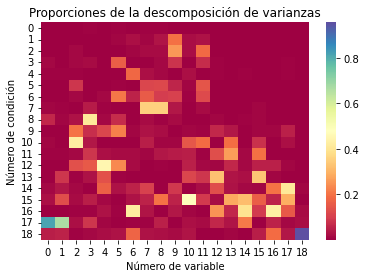
\includegraphics[width=\linewidth]{Images/VDM_adjusted.png}
            \caption{Proporción de descomposición de varianzas incluyendo también la región que se encuentran.}
        \end{subfigure}
        \caption{Análisis de descomposición de las varianzas en términos de los números de condición.}\label{fig:pis}
    \end{figure}

    Una vez hecho este análisis, entonces puede construirse el modelo. Para poder 
    imputar los datos faltantes, se propone usar una técnica de k-vecinos más cercanos,
    que aunque bien no se conocen los efectos de esta técnica en la estructura 
    inherente de los datos \cite{beretta_nearest_2016}, tienden a mejorar las 
    propiedades inferenciales de los datos. Después de este preprocesamiento, 
    se construyen los siguientes modelos:

    \begin{enumerate}
        \item Regresión Ridge: se hace validación cruzada para ajustar el parámetro de regularización $\lambda$.
        \item Regresión lineal: se hace de manera ordinaria. 
        \item Regresión Lasso: se hace validación cruzada para ajustar el parámetro de regularización $\lambda$.
    \end{enumerate}

    Después de construidos, se corren 20 veces los experimentos y se calculan 
    sus errores cuadráticos medios para poder compararlos. Adicionalmente, se 
    observan las distribuciones de los residuales en la figura \ref{fig:residuals}

    \begin{table}[h!]
        \centering
        \caption{Resultados de regresiones}
        \begin{tabular}{r c c c}
            \hline
            Valor & Ridge & OLS & Lasso \\
            \hline \hline
            
            $\lambda$ & 2.637 & – & 0.039 \\
            \hline 
            $R^2$ en todos los datos & 0.879 & 0.881 & 0.879 \\
            \hline
            $MSE$ entrenamiento & 13.45 & 12.99 & 13.34 \\
            \hline
            $MSE$ prueba & 18.85 & 19.34 & 18.40 \\
            \hline
        \end{tabular}
    \end{table}

    Se puede observar que todos los modelos tienen un rendimiento relativamente cercano, 
    siendo muy ligeramente menores los valores del error cuadrático medio en los 
    datos de prueba para la regresión Ridge y Lasso. Observando la figura \ref{fig:residuals}
    \begin{figure}
        \centering
        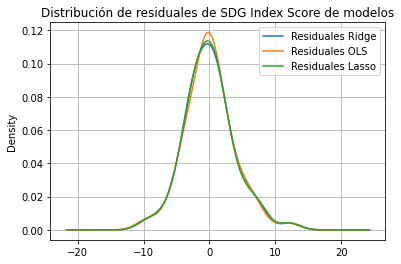
\includegraphics[width=0.8\linewidth]{Images/Residuals.png}
        \caption{Distribución de residuales de cada uno de los modelos. Puede observarse son muy similares, y son relativamente normales.}\label{fig:residuals}
    \end{figure}

    \section{Conclusiones}

    \section{Referencias}
    \printbibliography

\end{document}